\documentclass{article} % For LaTeX2e
\usepackage{nips13submit_e,times}
\usepackage{hyperref}
\usepackage{url}
\usepackage{graphicx}
\usepackage{subfig}

\title{Object Recognition using CALTECH 256 Dataset}


\author{
Anubhab Majumdar \\
\texttt{amajumd@ncsu.edu} \\
\And
Toshal Phene \\
\texttt{tphene@ncsu.edu} \\
\AND
Shubham Munot \\
\texttt{samunot@ncsu.edu} \\
}

% The \author macro works with any number of authors. There are two commands
% used to separate the names and addresses of multiple authors: \And and \AND.
%
% Using \And between authors leaves it to \LaTeX{} to determine where to break
% the lines. Using \AND forces a linebreak at that point. So, if \LaTeX{}
% puts 3 of 4 authors names on the first line, and the last on the second
% line, try using \AND instead of \And before the third author name.

\newcommand{\fix}{\marginpar{FIX}}
\newcommand{\new}{\marginpar{NEW}}

\nipsfinalcopy % Uncomment for camera-ready version

\begin{document}


\maketitle


\section{Introduction}
Object recognition is a quintessential machine learning problem of modern times. It is difficult for machines to recognize a large variety of objects in different conditions of lighting, occlusion and skew. In recent years, this field has seen huge leaps with machines becoming adept at object recognition. In this project, we explore different approaches of tackling this problem

\par We are using the CALTECH 256 dataset \href{http://www.vision.caltech.edu/Image_Datasets/Caltech256/}{(link)} for object recognition \cite{caltech_dataset_paper}. The dataset has 256 unique categories of images. The number of samples in each category varies from 80 to over 200. This dataset is quite a standard dataset in the field of object recognition and has been been used in important research papers like \cite{knn_svm_paper}. Our goal is to train a machine learning algorithm using 80\% of the data and test using the remaining 20\%. We experimented on a small subset (4-5 categories) of the dataset. 

\par The experiments have been implemented using student version of MATLAB and python/tensorflow. Some of the less computationally intensive models are trained on personal computers, while the deep networks are trained on VCL servers.


\section{Methodology}

A typical classification system is shown in Fig.\ref{fig:basic_system}. The paper focuses on the machine learning block shown in Fig.\ref{fig:basic_system}. Different learning algorithms ranging from simple and lazy methods like KNN to deep convolution neural network is applied and results are compared for a comprehensive understanding of which method works better. The paper also tries to draw conclusion as to why certain methods work better than others. 

\begin{figure}[h]
\centering
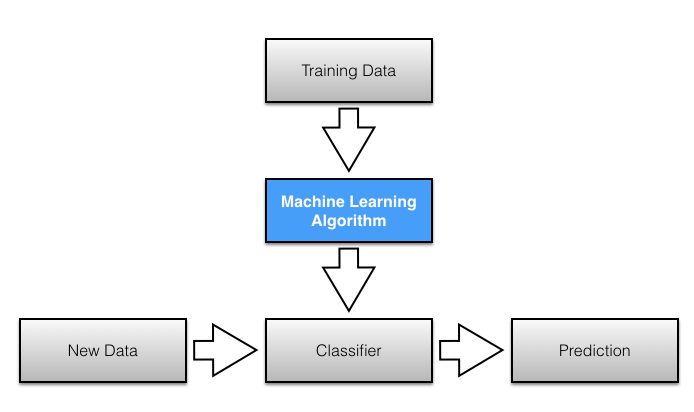
\includegraphics[scale=0.3]{learning_algorithm_basic.png}
\caption{A typical prediction system}
\label{fig:basic_system}
\end{figure}

Before jumping into the algorithms applied, let's talk about the data itself. We have chosen the following 4 categories for our experimentation:
\begin{itemize} 

\item
Backpack (Sample size - 151)
\item
Binoculars (Sample size - 216)
\item
Eiffel Tower (Sample size - 83)
\item
Fried egg (Sample size - 90)

\end{itemize}

Sample of some images from the dataset are shown in Fig.\ref{Fig:sample_dataset}.

\begin{figure}
\centering
\begin{tabular}{|c|c|c|c|}
\hline 
\subfloat{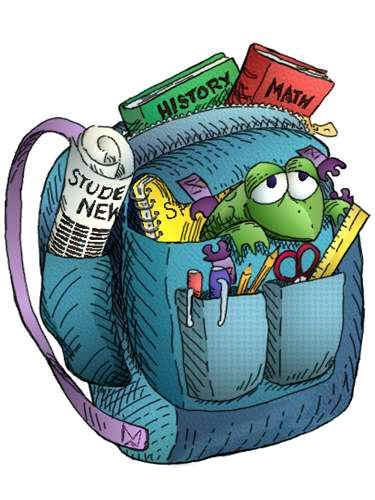
\includegraphics[scale = 0.05]{003_0001.jpg}} &
\subfloat{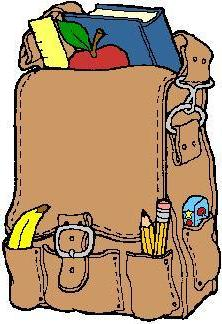
\includegraphics[scale = 0.05]{003_0002.jpg}} &
\subfloat{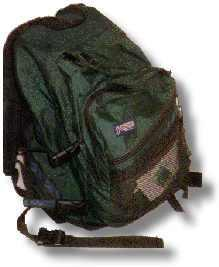
\includegraphics[scale = 0.05]{003_0003.jpg}} &
\subfloat{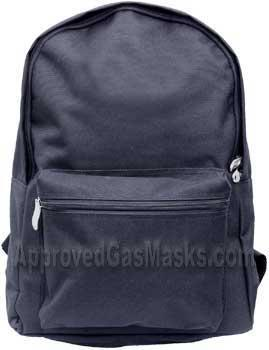
\includegraphics[scale = 0.05]{003_0004.jpg}}\\
\hline
\subfloat{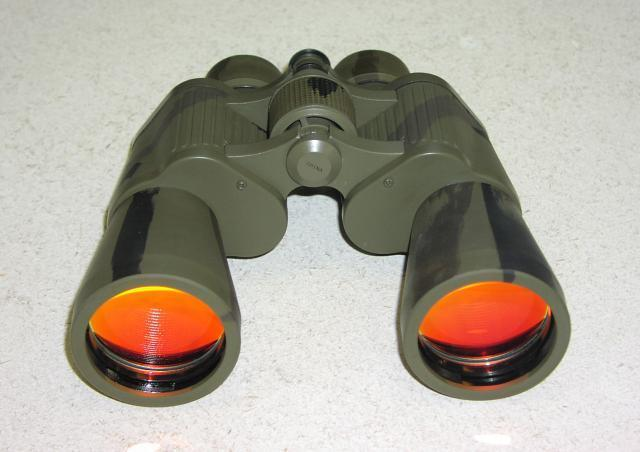
\includegraphics[scale = 0.05]{012_0001.jpg}} &
\subfloat{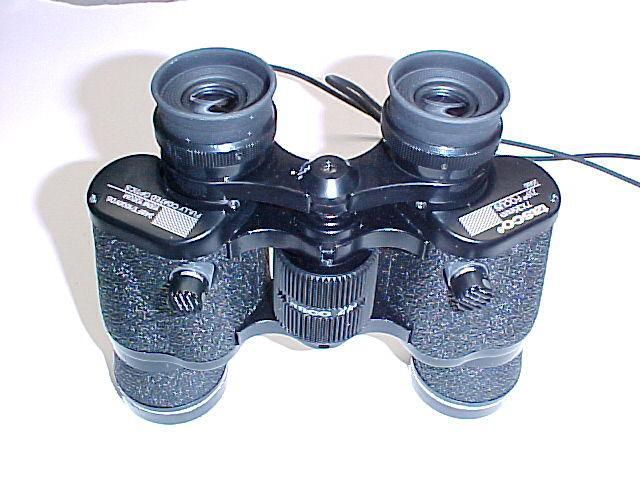
\includegraphics[scale = 0.05]{012_0002.jpg}} &
\subfloat{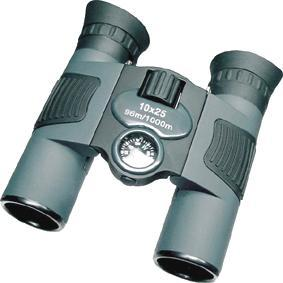
\includegraphics[scale = 0.05]{012_0003.jpg}} &
\subfloat{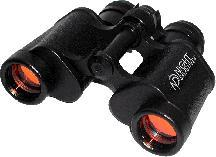
\includegraphics[scale = 0.05]{012_0004.jpg}}\\
\hline 
\subfloat{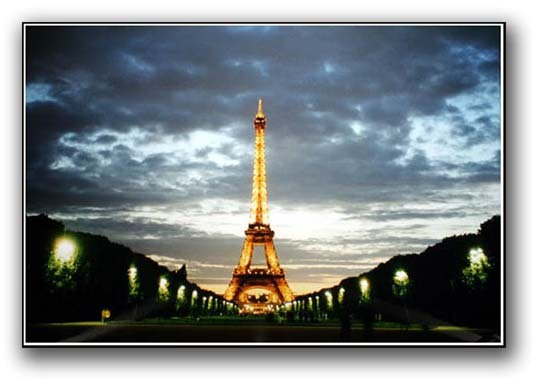
\includegraphics[scale = 0.05]{062_0001.jpg}} &
\subfloat{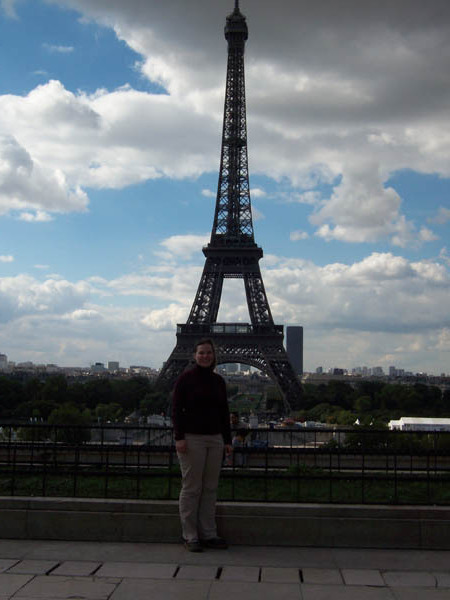
\includegraphics[scale = 0.05]{062_0002.jpg}} &
\subfloat{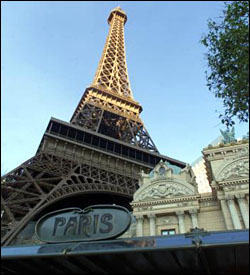
\includegraphics[scale = 0.05]{062_0003.jpg}} &
\subfloat{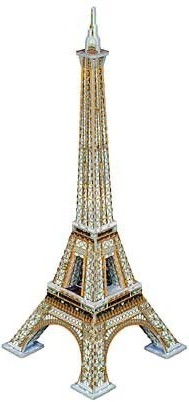
\includegraphics[scale = 0.05]{062_0004.jpg}}\\
\hline 
\subfloat{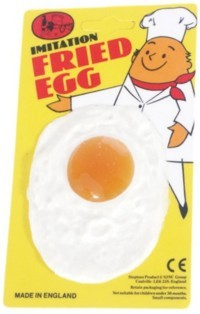
\includegraphics[scale = 0.05]{078_0001.jpg}} &
\subfloat{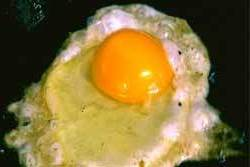
\includegraphics[scale = 0.05]{078_0002.jpg}} &
\subfloat{
\includegraphics[scale = 0.05]{078_0003.jpg}} &
\subfloat{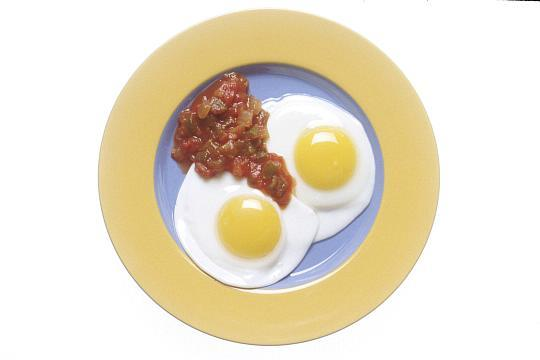
\includegraphics[scale = 0.05]{078_0004.jpg}}\\
\hline

\end{tabular}
\caption{Few samples from our dataset}
\label{Fig:sample_dataset}
\end{figure}

\subsection{KNN}
% write here

\subsection{SVM}
% write here


\subsection{Convolution Neural Network}


\section{Experiments and Results}

\subsection{KNN}
% write here


\subsection{SVM}
% write here


\subsection{Convolution Neural Network}



\section{Conclusion}




\begin{thebibliography}{9}

\bibitem{caltech_dataset_paper} 
Greg Griffin, Alex Holub and Pietro Perona. \\
\textit{Caltech-256 Object Category Dataset}. 
 
\bibitem{knn_svm_paper} 
Hao Zhang, Alexander C. Berg, Michael Maire and Jitendra Malik \\
\textit{SVM-KNN: Discriminative Nearest Neighbor Classification for Visual Category
Recognition}.

 
\bibitem{knuthwebsite} 
Knuth: Computers and Typesetting,
\\\texttt{http://www-cs-faculty.stanford.edu/\~{}uno/abcde.html}
\end{thebibliography}

\end{document}
